\subsection{Provide the arrays $\Phi$ and $\Lambda$ obtained using the Euler approximation method and the Matlab command \textit{c2d}.}
\subsubsection*{Euler approximation}
\begin{equation}
    \Phi = 
    \left[ {\begin{array}{ccccc}
        1 &0 &0   &0.1 &0     \\
        0 &1 &0.5 &0   &0     \\
        0 &0 &1   &0   &0.008 \\
        0 &0 &0   &0.9 &0     \\
        0 &0 &0   &0   &0.5   \\
    \end{array} } \right]    
    ,\quad
    \Lambda =
    \left[ {\begin{array}{cc}
        0 &0\\
        0 &0\\
        0 &0\\
        0.1 &0\\
        0 &0.5\\
    \end{array} } \right]
\end{equation}

\subsubsection*{Matlab \textit{c2d}}
\begin{equation}
    \Phi = 
    \left[ {\begin{array}{ccccc}
        1 &0 &0   &0.95  &0     \\
        0 &1 &0.5 &0     &0.002     \\
        0 &0 &1   &0     &0.006 \\
        0 &0 &0   &0.905 &0     \\
        0 &0 &0   &0     &0.607   \\
    \end{array} } \right]    
    ,\quad
    \Lambda =
    \left[ {\begin{array}{cc}
        0.005 &0\\
        0 &0\\
        0 &0.002\\
        0.095 &0\\
        0 &0.393\\
    \end{array} } \right]
\end{equation}



\subsection{Provide a screenshot of your implementation of the Non linear model - continuous time block.}

\begin{figure}[H]
    \centering
    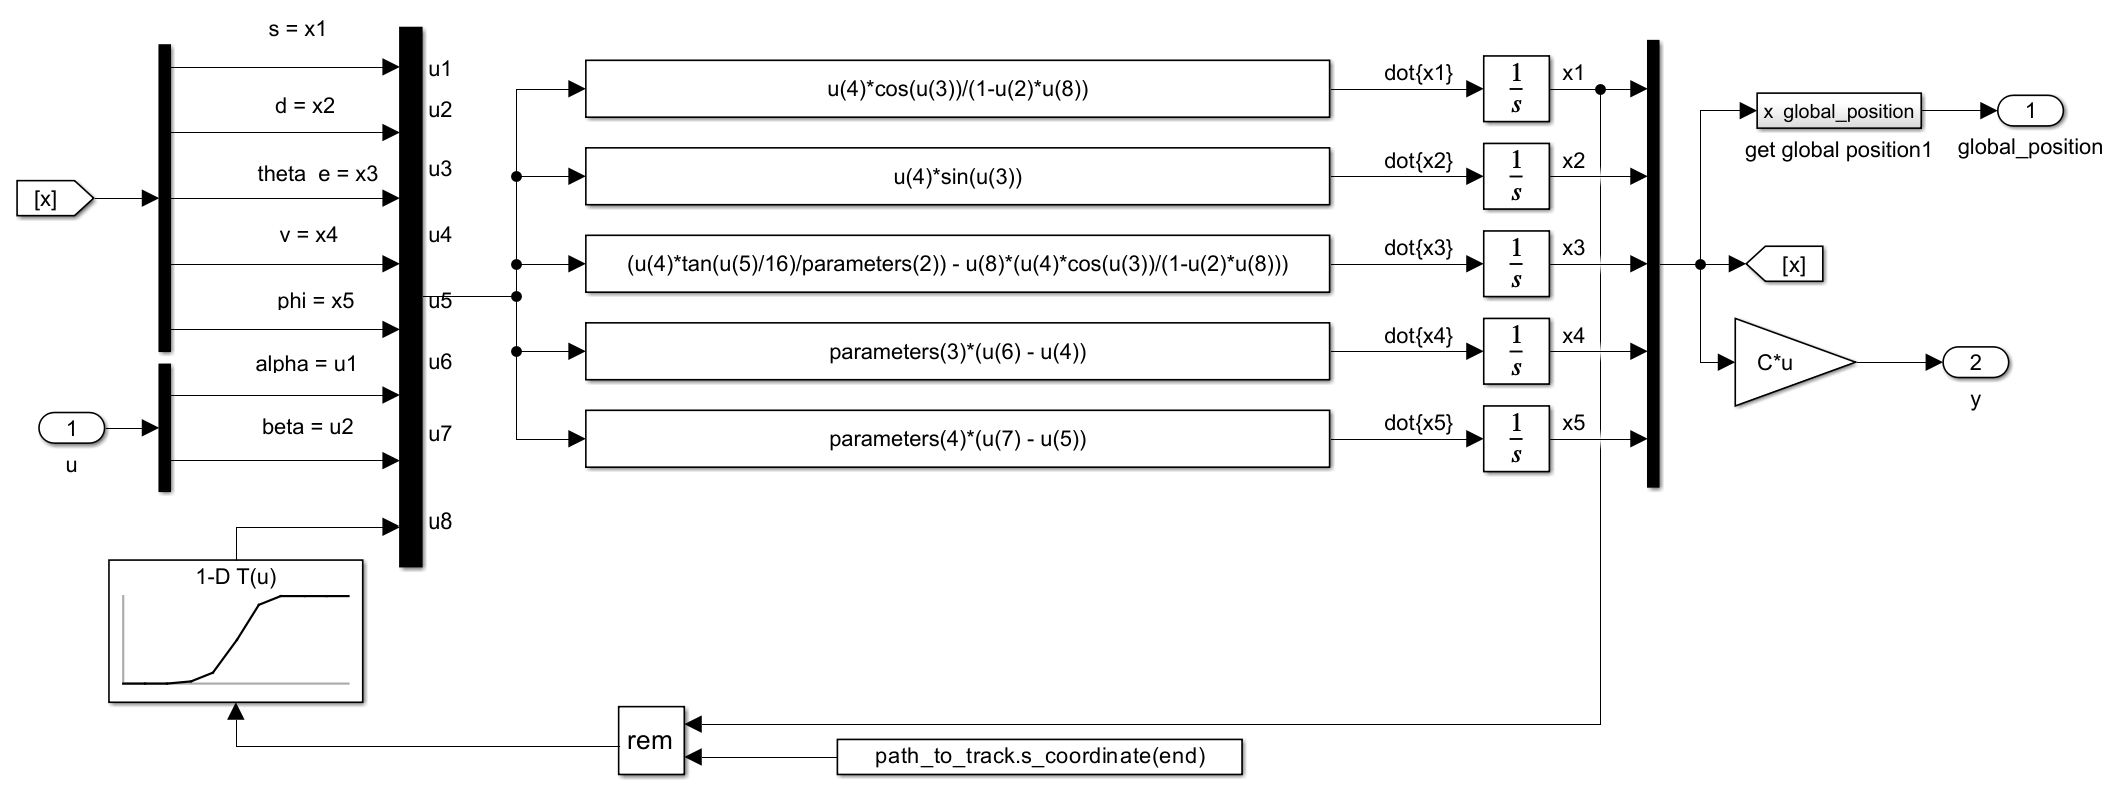
\includegraphics[width = 0.9\linewidth]{Latex report/image/nonLinModelContinousTime.png}
    \caption{Non linear model in continous time implementation in Simulink}
    \label{fig:continousTimeSimulink}
\end{figure}




\subsection{Provide a screenshot of the block diagram implemented in open loop experiments.slx.}
\begin{figure}
    \centering
    \includegraphics{}
    \caption{Caption}
    \label{fig:my_label}
\end{figure}





\subsection{Report the simulation results, including the information concerning the initial state you used, the sequence of inputs you applied, and the simulated results.}




\subsection{Does the linear model resemble sufficiently well the behavior obtained from the non-linear model? Why?}




\subsection{Do the results obtained using the discrete-time linear model resemble those obtained by the continuous-time linear model? What is then interesting about using the discrete-time linear model instead of the continuous-time linear model to design control strategies?}



